\documentclass[1p]{elsarticle_modified}
%\bibliographystyle{elsarticle-num}

%\usepackage[colorlinks]{hyperref}
%\usepackage{abbrmath_seonhwa} %\Abb, \Ascr, \Acal ,\Abf, \Afrak
\usepackage{amsfonts}
\usepackage{amssymb}
\usepackage{amsmath}
\usepackage{amsthm}
\usepackage{scalefnt}
\usepackage{amsbsy}
\usepackage{kotex}
\usepackage{caption}
\usepackage{subfig}
\usepackage{color}
\usepackage{graphicx}
\usepackage{xcolor} %% white, black, red, green, blue, cyan, magenta, yellow
\usepackage{float}
\usepackage{setspace}
\usepackage{hyperref}

\usepackage{tikz}
\usetikzlibrary{arrows}

\usepackage{multirow}
\usepackage{array} % fixed length table
\usepackage{hhline}

%%%%%%%%%%%%%%%%%%%%%
\makeatletter
\renewcommand*\env@matrix[1][\arraystretch]{%
	\edef\arraystretch{#1}%
	\hskip -\arraycolsep
	\let\@ifnextchar\new@ifnextchar
	\array{*\c@MaxMatrixCols c}}
\makeatother %https://tex.stackexchange.com/questions/14071/how-can-i-increase-the-line-spacing-in-a-matrix
%%%%%%%%%%%%%%%

\usepackage[normalem]{ulem}

\newcommand{\msout}[1]{\ifmmode\text{\sout{\ensuremath{#1}}}\else\sout{#1}\fi}
%SOURCE: \msout is \stkout macro in https://tex.stackexchange.com/questions/20609/strikeout-in-math-mode

\newcommand{\cancel}[1]{
	\ifmmode
	{\color{red}\msout{#1}}
	\else
	{\color{red}\sout{#1}}
	\fi
}

\newcommand{\add}[1]{
	{\color{blue}\uwave{#1}}
}

\newcommand{\replace}[2]{
	\ifmmode
	{\color{red}\msout{#1}}{\color{blue}\uwave{#2}}
	\else
	{\color{red}\sout{#1}}{\color{blue}\uwave{#2}}
	\fi
}

\newcommand{\Sol}{\mathcal{S}} %segment
\newcommand{\D}{D} %diagram
\newcommand{\A}{\mathcal{A}} %arc


%%%%%%%%%%%%%%%%%%%%%%%%%%%%%5 test

\def\sl{\operatorname{\textup{SL}}(2,\Cbb)}
\def\psl{\operatorname{\textup{PSL}}(2,\Cbb)}
\def\quan{\mkern 1mu \triangleright \mkern 1mu}

\theoremstyle{definition}
\newtheorem{thm}{Theorem}[section]
\newtheorem{prop}[thm]{Proposition}
\newtheorem{lem}[thm]{Lemma}
\newtheorem{ques}[thm]{Question}
\newtheorem{cor}[thm]{Corollary}
\newtheorem{defn}[thm]{Definition}
\newtheorem{exam}[thm]{Example}
\newtheorem{rmk}[thm]{Remark}
\newtheorem{alg}[thm]{Algorithm}

\newcommand{\I}{\sqrt{-1}}
\begin{document}

%\begin{frontmatter}
%
%\title{Boundary parabolic representations of knots up to 8 crossings}
%
%%% Group authors per affiliation:
%\author{Yunhi Cho} 
%\address{Department of Mathematics, University of Seoul, Seoul, Korea}
%\ead{yhcho@uos.ac.kr}
%
%
%\author{Seonhwa Kim} %\fnref{s_kim}}
%\address{Center for Geometry and Physics, Institute for Basic Science, Pohang, 37673, Korea}
%\ead{ryeona17@ibs.re.kr}
%
%\author{Hyuk Kim}
%\address{Department of Mathematical Sciences, Seoul National University, Seoul 08826, Korea}
%\ead{hyukkim@snu.ac.kr}
%
%\author{Seokbeom Yoon}
%\address{Department of Mathematical Sciences, Seoul National University, Seoul, 08826,  Korea}
%\ead{sbyoon15@snu.ac.kr}
%
%\begin{abstract}
%We find all boundary parabolic representation of knots up to 8 crossings.
%
%\end{abstract}
%\begin{keyword}
%    \MSC[2010] 57M25 
%\end{keyword}
%
%\end{frontmatter}

%\linenumbers
%\tableofcontents
%
\newcommand\colored[1]{\textcolor{white}{\rule[-0.35ex]{0.8em}{1.4ex}}\kern-0.8em\color{red} #1}%
%\newcommand\colored[1]{\textcolor{white}{ #1}\kern-2.17ex	\textcolor{white}{ #1}\kern-1.81ex	\textcolor{white}{ #1}\kern-2.15ex\color{red}#1	}

{\Large $\underline{12n_{0286}~(K12n_{0286})}$}

\setlength{\tabcolsep}{10pt}
\renewcommand{\arraystretch}{1.6}
\vspace{1cm}\begin{tabular}{m{100pt}>{\centering\arraybackslash}m{274pt}}
\multirow{5}{120pt}{
	\centering
	\includegraphics[width=112pt]{../../../GIT/diagram.site/Diagrams/png/2375_12n_0286.png}\\
\ \ \ A knot diagram\footnotemark}&
\allowdisplaybreaks
\textbf{Linearized knot diagam} \\
\cline{2-2}
 &
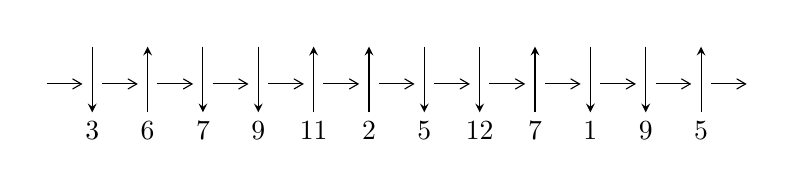
\begin{tikzpicture}[x=20pt, y=17pt]
	% nodes
	\node (C0) at (0, 0) {};
	\node (C1) at (1, 0) {};
	\node (C1U) at (1, +1) {};
	\node (C1D) at (1, -1) {3};

	\node (C2) at (2, 0) {};
	\node (C2U) at (2, +1) {};
	\node (C2D) at (2, -1) {6};

	\node (C3) at (3, 0) {};
	\node (C3U) at (3, +1) {};
	\node (C3D) at (3, -1) {7};

	\node (C4) at (4, 0) {};
	\node (C4U) at (4, +1) {};
	\node (C4D) at (4, -1) {9};

	\node (C5) at (5, 0) {};
	\node (C5U) at (5, +1) {};
	\node (C5D) at (5, -1) {11};

	\node (C6) at (6, 0) {};
	\node (C6U) at (6, +1) {};
	\node (C6D) at (6, -1) {2};

	\node (C7) at (7, 0) {};
	\node (C7U) at (7, +1) {};
	\node (C7D) at (7, -1) {5};

	\node (C8) at (8, 0) {};
	\node (C8U) at (8, +1) {};
	\node (C8D) at (8, -1) {12};

	\node (C9) at (9, 0) {};
	\node (C9U) at (9, +1) {};
	\node (C9D) at (9, -1) {7};

	\node (C10) at (10, 0) {};
	\node (C10U) at (10, +1) {};
	\node (C10D) at (10, -1) {1};

	\node (C11) at (11, 0) {};
	\node (C11U) at (11, +1) {};
	\node (C11D) at (11, -1) {9};

	\node (C12) at (12, 0) {};
	\node (C12U) at (12, +1) {};
	\node (C12D) at (12, -1) {5};
	\node (C13) at (13, 0) {};

	% arrows
	\draw[->,>={angle 60}]
	(C0) edge (C1) (C1) edge (C2) (C2) edge (C3) (C3) edge (C4) (C4) edge (C5) (C5) edge (C6) (C6) edge (C7) (C7) edge (C8) (C8) edge (C9) (C9) edge (C10) (C10) edge (C11) (C11) edge (C12) (C12) edge (C13) ;	\draw[->,>=stealth]
	(C1U) edge (C1D) (C2D) edge (C2U) (C3U) edge (C3D) (C4U) edge (C4D) (C5D) edge (C5U) (C6D) edge (C6U) (C7U) edge (C7D) (C8U) edge (C8D) (C9D) edge (C9U) (C10U) edge (C10D) (C11U) edge (C11D) (C12D) edge (C12U) ;
	\end{tikzpicture} \\
\hhline{~~} \\& 
\textbf{Solving Sequence} \\ \cline{2-2} 
 &
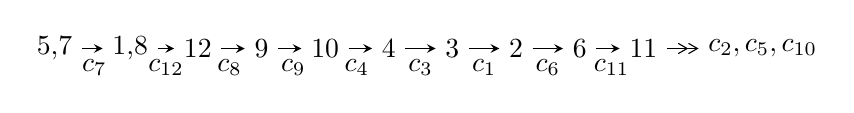
\begin{tikzpicture}[x=23pt, y=7pt]
	% node
	\node (A0) at (-1/8, 0) {5,7};
	\node (A1) at (17/16, 0) {1,8};
	\node (A2) at (17/8, 0) {12};
	\node (A3) at (25/8, 0) {9};
	\node (A4) at (33/8, 0) {10};
	\node (A5) at (41/8, 0) {4};
	\node (A6) at (49/8, 0) {3};
	\node (A7) at (57/8, 0) {2};
	\node (A8) at (65/8, 0) {6};
	\node (A9) at (73/8, 0) {11};
	\node (C1) at (1/2, -1) {$c_{7}$};
	\node (C2) at (13/8, -1) {$c_{12}$};
	\node (C3) at (21/8, -1) {$c_{8}$};
	\node (C4) at (29/8, -1) {$c_{9}$};
	\node (C5) at (37/8, -1) {$c_{4}$};
	\node (C6) at (45/8, -1) {$c_{3}$};
	\node (C7) at (53/8, -1) {$c_{1}$};
	\node (C8) at (61/8, -1) {$c_{6}$};
	\node (C9) at (69/8, -1) {$c_{11}$};
	\node (A10) at (11, 0) {$c_{2},c_{5},c_{10}$};

	% edge
	\draw[->,>=stealth]	
	(A0) edge (A1) (A1) edge (A2) (A2) edge (A3) (A3) edge (A4) (A4) edge (A5) (A5) edge (A6) (A6) edge (A7) (A7) edge (A8) (A8) edge (A9) ;
	\draw[->>,>={angle 60}]	
	(A9) edge (A10);
\end{tikzpicture} \\ 

\end{tabular} \\

\footnotetext{
The image of knot diagram is generated by the software ``\textbf{Draw programme}" developed by Andrew Bartholomew(\url{http://www.layer8.co.uk/maths/draw/index.htm\#Running-draw}), where we modified some parts for our purpose(\url{https://github.com/CATsTAILs/LinksPainter}).
}\phantom \\ \newline 
\centering \textbf{Ideals for irreducible components\footnotemark of $X_{\text{par}}$} 
 
\begin{align*}
I^u_{1}&=\langle 
-2.30879\times10^{95} u^{27}-4.77843\times10^{95} u^{26}+\cdots+2.74748\times10^{100} b+7.48326\times10^{100},\\
\phantom{I^u_{1}}&\phantom{= \langle  }3.53819\times10^{99} u^{27}+1.05291\times10^{100} u^{26}+\cdots+2.89208\times10^{105} a-7.68762\times10^{105},\\
\phantom{I^u_{1}}&\phantom{= \langle  }u^{28}+u^{27}+\cdots+29042 u+105263\rangle \\
I^u_{2}&=\langle 
-597082 u^{11}+1807096 u^{10}+\cdots+894777 b+933761,\\
\phantom{I^u_{2}}&\phantom{= \langle  }-3081635 u^{11}+7464402 u^{10}+\cdots+894777 a-1553044,\\
\phantom{I^u_{2}}&\phantom{= \langle  }u^{12}-2 u^{11}-2 u^{10}+10 u^9-10 u^8-22 u^7+45 u^6+78 u^5+82 u^4+52 u^3+22 u^2+6 u+1\rangle \\
I^u_{3}&=\langle 
b,\;a-1,\;u^4+u^3+2 u^2+2 u+1\rangle \\
I^u_{4}&=\langle 
b,\;a-1,\;u^2- u+1\rangle \\
\\
\end{align*}
\raggedright * 4 irreducible components of $\dim_{\mathbb{C}}=0$, with total 46 representations.\\
\footnotetext{All coefficients of polynomials are rational numbers. But the coefficients are sometimes approximated in decimal forms when there is not enough margin.}
\newpage
\renewcommand{\arraystretch}{1}
\centering \section*{I. $I^u_{1}= \langle -2.31\times10^{95} u^{27}-4.78\times10^{95} u^{26}+\cdots+2.75\times10^{100} b+7.48\times10^{100},\;3.54\times10^{99} u^{27}+1.05\times10^{100} u^{26}+\cdots+2.89\times10^{105} a-7.69\times10^{105},\;u^{28}+u^{27}+\cdots+29042 u+105263 \rangle$}
\flushleft \textbf{(i) Arc colorings}\\
\begin{tabular}{m{7pt} m{180pt} m{7pt} m{180pt} }
\flushright $a_{5}=$&$\begin{pmatrix}0\\u\end{pmatrix}$ \\
\flushright $a_{7}=$&$\begin{pmatrix}1\\0\end{pmatrix}$ \\
\flushright $a_{1}=$&$\begin{pmatrix}-1.22341\times10^{-6} u^{27}-3.64067\times10^{-6} u^{26}+\cdots+1.61930 u+2.65817\\8.40330\times10^{-6} u^{27}+0.0000173921 u^{26}+\cdots-1.76837 u-2.72368\end{pmatrix}$ \\
\flushright $a_{8}=$&$\begin{pmatrix}1\\u^2\end{pmatrix}$ \\
\flushright $a_{12}=$&$\begin{pmatrix}-1.22341\times10^{-6} u^{27}-3.64067\times10^{-6} u^{26}+\cdots+1.61930 u+2.65817\\8.28315\times10^{-6} u^{27}+0.0000219622 u^{26}+\cdots-1.56939 u-2.46924\end{pmatrix}$ \\
\flushright $a_{9}=$&$\begin{pmatrix}2.12062\times10^{-6} u^{27}+0.0000167463 u^{26}+\cdots-1.35559 u-0.0779815\\8.91847\times10^{-6} u^{27}+6.73686\times10^{-6} u^{26}+\cdots-0.963436 u-1.82371\end{pmatrix}$ \\
\flushright $a_{10}=$&$\begin{pmatrix}0.0000110391 u^{27}+0.0000234832 u^{26}+\cdots-2.31902 u-1.90169\\8.91847\times10^{-6} u^{27}+6.73686\times10^{-6} u^{26}+\cdots-0.963436 u-1.82371\end{pmatrix}$ \\
\flushright $a_{4}=$&$\begin{pmatrix}0.0000405549 u^{27}+0.0000479060 u^{26}+\cdots-5.29456 u-0.938872\\-0.0000209981 u^{27}-0.0000223788 u^{26}+\cdots+0.490410 u-0.198573\end{pmatrix}$ \\
\flushright $a_{3}=$&$\begin{pmatrix}0.0000195568 u^{27}+0.0000255272 u^{26}+\cdots-4.80415 u-1.13744\\-0.0000209981 u^{27}-0.0000223788 u^{26}+\cdots+0.490410 u-0.198573\end{pmatrix}$ \\
\flushright $a_{2}=$&$\begin{pmatrix}-2.70625\times10^{-6} u^{27}-0.0000166750 u^{26}+\cdots+3.86512 u+0.922256\\0.0000108644 u^{27}+0.0000140068 u^{26}+\cdots-0.974007 u+1.33386\end{pmatrix}$ \\
\flushright $a_{6}=$&$\begin{pmatrix}-0.0000225051 u^{27}-0.0000303714 u^{26}+\cdots+5.43569 u+0.658137\\0.0000146235 u^{27}+0.0000153805 u^{26}+\cdots-0.424743 u+0.764753\end{pmatrix}$ \\
\flushright $a_{11}=$&$\begin{pmatrix}5.66037\times10^{-6} u^{27}+0.0000117298 u^{26}+\cdots-1.06635 u-2.99223\\6.60870\times10^{-6} u^{27}+0.0000101990 u^{26}+\cdots-0.224821 u+1.16081\end{pmatrix}$\\&\end{tabular}
\flushleft \textbf{(ii) Obstruction class $= -1$}\\~\\
\flushleft \textbf{(iii) Cusp Shapes $= -0.0000493674 u^{27}-0.0000112265 u^{26}+\cdots+11.2065 u+0.643499$}\\~\\
\newpage\renewcommand{\arraystretch}{1}
\flushleft \textbf{(iv) u-Polynomials at the component}\newline \\
\begin{tabular}{m{50pt}|m{274pt}}
Crossings & \hspace{64pt}u-Polynomials at each crossing \\
\hline $$\begin{aligned}c_{1}\end{aligned}$$&$\begin{aligned}
&u^{28}+12 u^{27}+\cdots+19 u+4
\end{aligned}$\\
\hline $$\begin{aligned}c_{2},c_{6}\end{aligned}$$&$\begin{aligned}
&u^{28}+2 u^{27}+\cdots+5 u+2
\end{aligned}$\\
\hline $$\begin{aligned}c_{3}\end{aligned}$$&$\begin{aligned}
&u^{28}-2 u^{27}+\cdots+64 u+16
\end{aligned}$\\
\hline $$\begin{aligned}c_{4}\end{aligned}$$&$\begin{aligned}
&u^{28}+u^{27}+\cdots-122 u+17
\end{aligned}$\\
\hline $$\begin{aligned}c_{5}\end{aligned}$$&$\begin{aligned}
&u^{28}+u^{27}+\cdots-68 u+17
\end{aligned}$\\
\hline $$\begin{aligned}c_{7}\end{aligned}$$&$\begin{aligned}
&u^{28}+u^{27}+\cdots+29042 u+105263
\end{aligned}$\\
\hline $$\begin{aligned}c_{8},c_{11}\end{aligned}$$&$\begin{aligned}
&u^{28}-5 u^{27}+\cdots+613 u+1274
\end{aligned}$\\
\hline $$\begin{aligned}c_{9}\end{aligned}$$&$\begin{aligned}
&u^{28}+13 u^{27}+\cdots-12374 u+2437
\end{aligned}$\\
\hline $$\begin{aligned}c_{10}\end{aligned}$$&$\begin{aligned}
&u^{28}-7 u^{27}+\cdots+1306 u+37
\end{aligned}$\\
\hline $$\begin{aligned}c_{12}\end{aligned}$$&$\begin{aligned}
&u^{28}-3 u^{27}+\cdots+180 u+73
\end{aligned}$\\
\hline
\end{tabular}\\~\\
\newpage\renewcommand{\arraystretch}{1}
\flushleft \textbf{(v) Riley Polynomials at the component}\newline \\
\begin{tabular}{m{50pt}|m{274pt}}
Crossings & \hspace{64pt}Riley Polynomials at each crossing \\
\hline $$\begin{aligned}c_{1}\end{aligned}$$&$\begin{aligned}
&y^{28}+8 y^{27}+\cdots+191 y+16
\end{aligned}$\\
\hline $$\begin{aligned}c_{2},c_{6}\end{aligned}$$&$\begin{aligned}
&y^{28}+12 y^{27}+\cdots+19 y+4
\end{aligned}$\\
\hline $$\begin{aligned}c_{3}\end{aligned}$$&$\begin{aligned}
&y^{28}+4 y^{27}+\cdots+256 y+256
\end{aligned}$\\
\hline $$\begin{aligned}c_{4}\end{aligned}$$&$\begin{aligned}
&y^{28}+49 y^{27}+\cdots-4718 y+289
\end{aligned}$\\
\hline $$\begin{aligned}c_{5}\end{aligned}$$&$\begin{aligned}
&y^{28}-3 y^{27}+\cdots-1326 y+289
\end{aligned}$\\
\hline $$\begin{aligned}c_{7}\end{aligned}$$&$\begin{aligned}
&y^{28}+89 y^{27}+\cdots-103896967394 y+11080299169
\end{aligned}$\\
\hline $$\begin{aligned}c_{8},c_{11}\end{aligned}$$&$\begin{aligned}
&y^{28}+51 y^{27}+\cdots+22472147 y+1623076
\end{aligned}$\\
\hline $$\begin{aligned}c_{9}\end{aligned}$$&$\begin{aligned}
&y^{28}-61 y^{27}+\cdots-43826174 y+5938969
\end{aligned}$\\
\hline $$\begin{aligned}c_{10}\end{aligned}$$&$\begin{aligned}
&y^{28}+41 y^{27}+\cdots-885642 y+1369
\end{aligned}$\\
\hline $$\begin{aligned}c_{12}\end{aligned}$$&$\begin{aligned}
&y^{28}-69 y^{27}+\cdots+39870 y+5329
\end{aligned}$\\
\hline
\end{tabular}\\~\\
\newpage\flushleft \textbf{(vi) Complex Volumes and Cusp Shapes}
$$\begin{array}{c|c|c}  
\text{Solutions to }I^u_{1}& \I (\text{vol} + \sqrt{-1}CS) & \text{Cusp shape}\\
 \hline 
\begin{aligned}
u &= \phantom{-}1.121690 + 0.166562 I \\
a &= -0.309380 + 0.530304 I \\
b &= \phantom{-}0.595060 + 0.738659 I\end{aligned}
 & -2.29476 - 5.76614 I & -7.02724 + 7.83201 I \\ \hline\begin{aligned}
u &= \phantom{-}1.121690 - 0.166562 I \\
a &= -0.309380 - 0.530304 I \\
b &= \phantom{-}0.595060 - 0.738659 I\end{aligned}
 & -2.29476 + 5.76614 I & -7.02724 - 7.83201 I \\ \hline\begin{aligned}
u &= -0.500208 + 0.695651 I \\
a &= \phantom{-}0.484337 - 0.272007 I \\
b &= -0.109132 - 0.472868 I\end{aligned}
 & \phantom{-}0.024558 + 1.375320 I & -0.33642 - 5.32848 I \\ \hline\begin{aligned}
u &= -0.500208 - 0.695651 I \\
a &= \phantom{-}0.484337 + 0.272007 I \\
b &= -0.109132 + 0.472868 I\end{aligned}
 & \phantom{-}0.024558 - 1.375320 I & -0.33642 + 5.32848 I \\ \hline\begin{aligned}
u &= -0.723454 + 0.279934 I \\
a &= -0.021317 - 0.702292 I \\
b &= \phantom{-}0.371378 - 0.564796 I\end{aligned}
 & -0.40304 + 1.51323 I & -3.09504 - 4.74756 I \\ \hline\begin{aligned}
u &= -0.723454 - 0.279934 I \\
a &= -0.021317 + 0.702292 I \\
b &= \phantom{-}0.371378 + 0.564796 I\end{aligned}
 & -0.40304 - 1.51323 I & -3.09504 + 4.74756 I \\ \hline\begin{aligned}
u &= \phantom{-}0.600783 + 0.435618 I \\
a &= -0.863994 - 0.714884 I \\
b &= \phantom{-}0.764412 - 0.323762 I\end{aligned}
 & -3.61300 - 0.81317 I & -11.74702 + 0.23139 I \\ \hline\begin{aligned}
u &= \phantom{-}0.600783 - 0.435618 I \\
a &= -0.863994 + 0.714884 I \\
b &= \phantom{-}0.764412 + 0.323762 I\end{aligned}
 & -3.61300 + 0.81317 I & -11.74702 - 0.23139 I \\ \hline\begin{aligned}
u &= \phantom{-}0.647360 + 0.238923 I \\
a &= \phantom{-}0.876544 - 0.656944 I \\
b &= -0.330900 + 1.274360 I\end{aligned}
 & \phantom{-}5.75419 - 1.55004 I & \phantom{-}3.99662 + 0.73447 I \\ \hline\begin{aligned}
u &= \phantom{-}0.647360 - 0.238923 I \\
a &= \phantom{-}0.876544 + 0.656944 I \\
b &= -0.330900 - 1.274360 I\end{aligned}
 & \phantom{-}5.75419 + 1.55004 I & \phantom{-}3.99662 - 0.73447 I\\
 \hline 
 \end{array}$$\newpage$$\begin{array}{c|c|c}  
\text{Solutions to }I^u_{1}& \I (\text{vol} + \sqrt{-1}CS) & \text{Cusp shape}\\
 \hline 
\begin{aligned}
u &= -1.055570 + 0.863909 I \\
a &= \phantom{-}0.525304 - 0.025593 I \\
b &= -0.600723 - 0.856166 I\end{aligned}
 & \phantom{-}0.042186 + 1.135200 I & -1.07637 - 1.79124 I \\ \hline\begin{aligned}
u &= -1.055570 - 0.863909 I \\
a &= \phantom{-}0.525304 + 0.025593 I \\
b &= -0.600723 + 0.856166 I\end{aligned}
 & \phantom{-}0.042186 - 1.135200 I & -1.07637 + 1.79124 I \\ \hline\begin{aligned}
u &= -0.501357 + 0.390582 I \\
a &= \phantom{-}0.349177 + 0.948601 I \\
b &= -0.232725 - 1.265600 I\end{aligned}
 & \phantom{-}4.40104 + 6.85882 I & \phantom{-}1.45906 - 6.07740 I \\ \hline\begin{aligned}
u &= -0.501357 - 0.390582 I \\
a &= \phantom{-}0.349177 - 0.948601 I \\
b &= -0.232725 + 1.265600 I\end{aligned}
 & \phantom{-}4.40104 - 6.85882 I & \phantom{-}1.45906 + 6.07740 I \\ \hline\begin{aligned}
u &= \phantom{-}1.41576 + 0.06600 I \\
a &= \phantom{-}0.768140 + 0.147819 I \\
b &= -0.65731 + 1.30176 I\end{aligned}
 & \phantom{-}4.65876 + 1.17367 I & \phantom{-}4.17772 - 0.51764 I \\ \hline\begin{aligned}
u &= \phantom{-}1.41576 - 0.06600 I \\
a &= \phantom{-}0.768140 - 0.147819 I \\
b &= -0.65731 - 1.30176 I\end{aligned}
 & \phantom{-}4.65876 - 1.17367 I & \phantom{-}4.17772 + 0.51764 I \\ \hline\begin{aligned}
u &= -1.94268 + 0.04442 I \\
a &= \phantom{-}0.638810 - 0.235824 I \\
b &= -0.83183 - 1.35611 I\end{aligned}
 & \phantom{-}2.41032 - 6.19363 I & \phantom{-}1.11878 + 5.14377 I \\ \hline\begin{aligned}
u &= -1.94268 - 0.04442 I \\
a &= \phantom{-}0.638810 + 0.235824 I \\
b &= -0.83183 + 1.35611 I\end{aligned}
 & \phantom{-}2.41032 + 6.19363 I & \phantom{-}1.11878 - 5.14377 I \\ \hline\begin{aligned}
u &= \phantom{-}0.09793 + 2.80940 I \\
a &= \phantom{-}0.136557 - 0.869531 I \\
b &= -0.31138 - 1.92352 I\end{aligned}
 & \phantom{-}15.5072 + 3.1427 I & \phantom{-0.000000 } 0 \\ \hline\begin{aligned}
u &= \phantom{-}0.09793 - 2.80940 I \\
a &= \phantom{-}0.136557 + 0.869531 I \\
b &= -0.31138 + 1.92352 I\end{aligned}
 & \phantom{-}15.5072 - 3.1427 I & \phantom{-0.000000 } 0\\
 \hline 
 \end{array}$$\newpage$$\begin{array}{c|c|c}  
\text{Solutions to }I^u_{1}& \I (\text{vol} + \sqrt{-1}CS) & \text{Cusp shape}\\
 \hline 
\begin{aligned}
u &= -0.07521 + 3.00511 I \\
a &= \phantom{-}0.107635 + 0.836138 I \\
b &= -0.29648 + 1.95384 I\end{aligned}
 & \phantom{-}17.1357 + 2.5929 I & \phantom{-0.000000 } 0 \\ \hline\begin{aligned}
u &= -0.07521 - 3.00511 I \\
a &= \phantom{-}0.107635 - 0.836138 I \\
b &= -0.29648 - 1.95384 I\end{aligned}
 & \phantom{-}17.1357 - 2.5929 I & \phantom{-0.000000 } 0 \\ \hline\begin{aligned}
u &= \phantom{-}0.39997 + 3.28123 I \\
a &= \phantom{-}0.128139 - 0.754642 I \\
b &= -0.33448 - 2.02071 I\end{aligned}
 & \phantom{-}10.62630 - 4.32257 I & \phantom{-0.000000 } 0 \\ \hline\begin{aligned}
u &= \phantom{-}0.39997 - 3.28123 I \\
a &= \phantom{-}0.128139 + 0.754642 I \\
b &= -0.33448 + 2.02071 I\end{aligned}
 & \phantom{-}10.62630 + 4.32257 I & \phantom{-0.000000 } 0 \\ \hline\begin{aligned}
u &= -0.08895 + 3.46874 I \\
a &= \phantom{-}0.063138 + 0.756807 I \\
b &= -0.26759 + 2.03266 I\end{aligned}
 & \phantom{-}16.6423 + 6.6674 I & \phantom{-0.000000 } 0 \\ \hline\begin{aligned}
u &= -0.08895 - 3.46874 I \\
a &= \phantom{-}0.063138 - 0.756807 I \\
b &= -0.26759 - 2.03266 I\end{aligned}
 & \phantom{-}16.6423 - 6.6674 I & \phantom{-0.000000 } 0 \\ \hline\begin{aligned}
u &= \phantom{-}0.10393 + 3.63119 I \\
a &= \phantom{-}0.052461 - 0.730571 I \\
b &= -0.25830 - 2.06254 I\end{aligned}
 & \phantom{-}14.6448 - 12.3104 I & \phantom{-0.000000 } 0 \\ \hline\begin{aligned}
u &= \phantom{-}0.10393 - 3.63119 I \\
a &= \phantom{-}0.052461 + 0.730571 I \\
b &= -0.25830 + 2.06254 I\end{aligned}
 & \phantom{-}14.6448 + 12.3104 I & \phantom{-0.000000 } 0\\
 \hline 
 \end{array}$$\newpage\newpage\renewcommand{\arraystretch}{1}
\centering \section*{II. $I^u_{2}= \langle -5.97\times10^{5} u^{11}+1.81\times10^{6} u^{10}+\cdots+8.95\times10^{5} b+9.34\times10^{5},\;-3.08\times10^{6} u^{11}+7.46\times10^{6} u^{10}+\cdots+8.95\times10^{5} a-1.55\times10^{6},\;u^{12}-2 u^{11}+\cdots+6 u+1 \rangle$}
\flushleft \textbf{(i) Arc colorings}\\
\begin{tabular}{m{7pt} m{180pt} m{7pt} m{180pt} }
\flushright $a_{5}=$&$\begin{pmatrix}0\\u\end{pmatrix}$ \\
\flushright $a_{7}=$&$\begin{pmatrix}1\\0\end{pmatrix}$ \\
\flushright $a_{1}=$&$\begin{pmatrix}3.44403 u^{11}-8.34219 u^{10}+\cdots+18.7046 u+1.73568\\0.667297 u^{11}-2.01960 u^{10}+\cdots-4.48583 u-1.04357\end{pmatrix}$ \\
\flushright $a_{8}=$&$\begin{pmatrix}1\\u^2\end{pmatrix}$ \\
\flushright $a_{12}=$&$\begin{pmatrix}3.44403 u^{11}-8.34219 u^{10}+\cdots+18.7046 u+1.73568\\0.878181 u^{11}-2.42594 u^{10}+\cdots+0.794990 u+0.410573\end{pmatrix}$ \\
\flushright $a_{9}=$&$\begin{pmatrix}2.27082 u^{11}-4.73048 u^{10}+\cdots+28.1706 u+3.21957\\0.667297 u^{11}-2.01960 u^{10}+\cdots-4.48583 u-2.04357\end{pmatrix}$ \\
\flushright $a_{10}=$&$\begin{pmatrix}2.93811 u^{11}-6.75008 u^{10}+\cdots+23.6848 u+1.17600\\0.667297 u^{11}-2.01960 u^{10}+\cdots-4.48583 u-2.04357\end{pmatrix}$ \\
\flushright $a_{4}=$&$\begin{pmatrix}u^{11}-2 u^{10}+\cdots+22 u+6\\1.45414 u^{11}-3.11917 u^{10}+\cdots+19.9285 u+3.44403\end{pmatrix}$ \\
\flushright $a_{3}=$&$\begin{pmatrix}2.45414 u^{11}-5.11917 u^{10}+\cdots+41.9285 u+9.44403\\1.45414 u^{11}-3.11917 u^{10}+\cdots+19.9285 u+3.44403\end{pmatrix}$ \\
\flushright $a_{2}=$&$\begin{pmatrix}0.230870 u^{11}-0.441754 u^{10}+\cdots+7.11887 u+3.22327\\0.230870 u^{11}-0.441754 u^{10}+\cdots+7.11887 u+2.22327\end{pmatrix}$ \\
\flushright $a_{6}=$&$\begin{pmatrix}u^{11}-2 u^{10}+\cdots+22 u+6\\0.769130 u^{11}-1.55825 u^{10}+\cdots+14.8811 u+2.77673\end{pmatrix}$ \\
\flushright $a_{11}=$&$\begin{pmatrix}2.27082 u^{11}-4.73048 u^{10}+\cdots+28.1706 u+3.21957\\1.00165 u^{11}-2.54029 u^{10}+\cdots+1.93274 u-0.778272\end{pmatrix}$\\&\end{tabular}
\flushleft \textbf{(ii) Obstruction class $= 1$}\\~\\
\flushleft \textbf{(iii) Cusp Shapes $= \frac{2135288}{894777} u^{11}-\frac{2175584}{298259} u^{10}+\cdots-\frac{5146736}{298259} u-\frac{4858220}{894777}$}\\~\\
\newpage\renewcommand{\arraystretch}{1}
\flushleft \textbf{(iv) u-Polynomials at the component}\newline \\
\begin{tabular}{m{50pt}|m{274pt}}
Crossings & \hspace{64pt}u-Polynomials at each crossing \\
\hline $$\begin{aligned}c_{1}\end{aligned}$$&$\begin{aligned}
&(u^6-3 u^5+5 u^4-4 u^3+2 u^2- u+1)^2
\end{aligned}$\\
\hline $$\begin{aligned}c_{2},c_{6},c_{8}\\c_{11}\end{aligned}$$&$\begin{aligned}
&u^{12}+3 u^{10}+5 u^8+4 u^6+2 u^4+u^2+1
\end{aligned}$\\
\hline $$\begin{aligned}c_{3}\end{aligned}$$&$\begin{aligned}
&u^{12}- u^{10}+5 u^8+6 u^4-3 u^2+1
\end{aligned}$\\
\hline $$\begin{aligned}c_{4},c_{5}\end{aligned}$$&$\begin{aligned}
&(u^2+1)^6
\end{aligned}$\\
\hline $$\begin{aligned}c_{7}\end{aligned}$$&$\begin{aligned}
&u^{12}-2 u^{11}+\cdots+6 u+1
\end{aligned}$\\
\hline $$\begin{aligned}c_{9}\end{aligned}$$&$\begin{aligned}
&u^{12}-12 u^{11}+\cdots-116 u+17
\end{aligned}$\\
\hline $$\begin{aligned}c_{10}\end{aligned}$$&$\begin{aligned}
&u^{12}-6 u^{11}+\cdots+2 u+1
\end{aligned}$\\
\hline $$\begin{aligned}c_{12}\end{aligned}$$&$\begin{aligned}
&u^{12}-2 u^{11}+\cdots-56 u+17
\end{aligned}$\\
\hline
\end{tabular}\\~\\
\newpage\renewcommand{\arraystretch}{1}
\flushleft \textbf{(v) Riley Polynomials at the component}\newline \\
\begin{tabular}{m{50pt}|m{274pt}}
Crossings & \hspace{64pt}Riley Polynomials at each crossing \\
\hline $$\begin{aligned}c_{1}\end{aligned}$$&$\begin{aligned}
&(y^6+y^5+5 y^4+6 y^2+3 y+1)^2
\end{aligned}$\\
\hline $$\begin{aligned}c_{2},c_{6},c_{8}\\c_{11}\end{aligned}$$&$\begin{aligned}
&(y^6+3 y^5+5 y^4+4 y^3+2 y^2+y+1)^2
\end{aligned}$\\
\hline $$\begin{aligned}c_{3}\end{aligned}$$&$\begin{aligned}
&(y^6- y^5+5 y^4+6 y^2-3 y+1)^2
\end{aligned}$\\
\hline $$\begin{aligned}c_{4},c_{5}\end{aligned}$$&$\begin{aligned}
&(y+1)^{12}
\end{aligned}$\\
\hline $$\begin{aligned}c_{7}\end{aligned}$$&$\begin{aligned}
&y^{12}-8 y^{11}+\cdots+8 y+1
\end{aligned}$\\
\hline $$\begin{aligned}c_{9}\end{aligned}$$&$\begin{aligned}
&y^{12}-6 y^{11}+\cdots+620 y+289
\end{aligned}$\\
\hline $$\begin{aligned}c_{10}\end{aligned}$$&$\begin{aligned}
&y^{12}+8 y^{11}+\cdots-8 y+1
\end{aligned}$\\
\hline $$\begin{aligned}c_{12}\end{aligned}$$&$\begin{aligned}
&y^{12}+6 y^{11}+\cdots-620 y+289
\end{aligned}$\\
\hline
\end{tabular}\\~\\
\newpage\flushleft \textbf{(vi) Complex Volumes and Cusp Shapes}
$$\begin{array}{c|c|c}  
\text{Solutions to }I^u_{2}& \I (\text{vol} + \sqrt{-1}CS) & \text{Cusp shape}\\
 \hline 
\begin{aligned}
u &= -0.140919 + 0.593678 I \\
a &= \phantom{-}0.372841 - 0.809839 I \\
b &= \phantom{-}0.664531 + 0.428243 I\end{aligned}
 & -1.89061 + 0.92430 I & -5.71672 - 0.79423 I \\ \hline\begin{aligned}
u &= -0.140919 - 0.593678 I \\
a &= \phantom{-}0.372841 + 0.809839 I \\
b &= \phantom{-}0.664531 - 0.428243 I\end{aligned}
 & -1.89061 - 0.92430 I & -5.71672 + 0.79423 I \\ \hline\begin{aligned}
u &= -0.409813 + 0.212587 I \\
a &= \phantom{-}1.22433 + 2.35408 I \\
b &= \phantom{-}0.295542 + 1.002190 I\end{aligned}
 & \phantom{-}1.89061 - 0.92430 I & \phantom{-}1.71672 + 0.79423 I \\ \hline\begin{aligned}
u &= -0.409813 - 0.212587 I \\
a &= \phantom{-}1.22433 - 2.35408 I \\
b &= \phantom{-}0.295542 - 1.002190 I\end{aligned}
 & \phantom{-}1.89061 + 0.92430 I & \phantom{-}1.71672 - 0.79423 I \\ \hline\begin{aligned}
u &= -0.126193 + 0.399916 I \\
a &= -1.77409 - 2.12563 I \\
b &= \phantom{-}0.558752 - 1.073950 I\end{aligned}
 & \phantom{-0.000000 -}5.69302 I & -2.00000 - 5.51057 I \\ \hline\begin{aligned}
u &= -0.126193 - 0.399916 I \\
a &= -1.77409 + 2.12563 I \\
b &= \phantom{-}0.558752 + 1.073950 I\end{aligned}
 & \phantom{-0.000000 } -5.69302 I & -2.00000 + 5.51057 I \\ \hline\begin{aligned}
u &= -1.59457 + 0.37850 I \\
a &= \phantom{-}0.777546 - 0.627907 I \\
b &= -0.295542 - 1.002190 I\end{aligned}
 & \phantom{-}1.89061 - 0.92430 I & \phantom{-}1.71672 + 0.79423 I \\ \hline\begin{aligned}
u &= -1.59457 - 0.37850 I \\
a &= \phantom{-}0.777546 + 0.627907 I \\
b &= -0.295542 + 1.002190 I\end{aligned}
 & \phantom{-}1.89061 + 0.92430 I & \phantom{-}1.71672 - 0.79423 I \\ \hline\begin{aligned}
u &= \phantom{-}0.99741 + 1.92274 I \\
a &= \phantom{-}0.773186 + 0.178358 I \\
b &= -0.664531 + 0.428243 I\end{aligned}
 & -1.89061 - 0.92430 I & -5.71672 + 0.79423 I \\ \hline\begin{aligned}
u &= \phantom{-}0.99741 - 1.92274 I \\
a &= \phantom{-}0.773186 - 0.178358 I \\
b &= -0.664531 - 0.428243 I\end{aligned}
 & -1.89061 + 0.92430 I & -5.71672 - 0.79423 I\\
 \hline 
 \end{array}$$\newpage$$\begin{array}{c|c|c}  
\text{Solutions to }I^u_{2}& \I (\text{vol} + \sqrt{-1}CS) & \text{Cusp shape}\\
 \hline 
\begin{aligned}
u &= \phantom{-}2.27409 + 0.71759 I \\
a &= \phantom{-}0.626193 + 0.487844 I \\
b &= -0.558752 + 1.073950 I\end{aligned}
 & \phantom{-0.000000 -}5.69302 I & -2.00000 - 5.51057 I \\ \hline\begin{aligned}
u &= \phantom{-}2.27409 - 0.71759 I \\
a &= \phantom{-}0.626193 - 0.487844 I \\
b &= -0.558752 - 1.073950 I\end{aligned}
 & \phantom{-0.000000 } -5.69302 I & -2.00000 + 5.51057 I\\
 \hline 
 \end{array}$$\newpage\newpage\renewcommand{\arraystretch}{1}
\centering \section*{III. $I^u_{3}= \langle b,\;a-1,\;u^4+u^3+2 u^2+2 u+1 \rangle$}
\flushleft \textbf{(i) Arc colorings}\\
\begin{tabular}{m{7pt} m{180pt} m{7pt} m{180pt} }
\flushright $a_{5}=$&$\begin{pmatrix}0\\u\end{pmatrix}$ \\
\flushright $a_{7}=$&$\begin{pmatrix}1\\0\end{pmatrix}$ \\
\flushright $a_{1}=$&$\begin{pmatrix}1\\0\end{pmatrix}$ \\
\flushright $a_{8}=$&$\begin{pmatrix}1\\u^2\end{pmatrix}$ \\
\flushright $a_{12}=$&$\begin{pmatrix}1\\u^2\end{pmatrix}$ \\
\flushright $a_{9}=$&$\begin{pmatrix}1\\u^2\end{pmatrix}$ \\
\flushright $a_{10}=$&$\begin{pmatrix}u^2+1\\u^2\end{pmatrix}$ \\
\flushright $a_{4}=$&$\begin{pmatrix}u\\u^3+u\end{pmatrix}$ \\
\flushright $a_{3}=$&$\begin{pmatrix}u^3+2 u\\u^3+u\end{pmatrix}$ \\
\flushright $a_{2}=$&$\begin{pmatrix}-2 u^3- u^2-3 u-1\\- u^3- u-1\end{pmatrix}$ \\
\flushright $a_{6}=$&$\begin{pmatrix}u\\u^3+u\end{pmatrix}$ \\
\flushright $a_{11}=$&$\begin{pmatrix}1\\u^2\end{pmatrix}$\\&\end{tabular}
\flushleft \textbf{(ii) Obstruction class $= -1$}\\~\\
\flushleft \textbf{(iii) Cusp Shapes $= -4 u^3-4 u-2$}\\~\\
\newpage\renewcommand{\arraystretch}{1}
\flushleft \textbf{(iv) u-Polynomials at the component}\newline \\
\begin{tabular}{m{50pt}|m{274pt}}
Crossings & \hspace{64pt}u-Polynomials at each crossing \\
\hline $$\begin{aligned}c_{1},c_{3}\end{aligned}$$&$\begin{aligned}
&(u^2+u+1)^2
\end{aligned}$\\
\hline $$\begin{aligned}c_{2},c_{6}\end{aligned}$$&$\begin{aligned}
&(u^2- u+1)^2
\end{aligned}$\\
\hline $$\begin{aligned}c_{4},c_{5},c_{7}\\c_{12}\end{aligned}$$&$\begin{aligned}
&u^4+u^3+2 u^2+2 u+1
\end{aligned}$\\
\hline $$\begin{aligned}c_{8},c_{11}\end{aligned}$$&$\begin{aligned}
&u^4
\end{aligned}$\\
\hline $$\begin{aligned}c_{9}\end{aligned}$$&$\begin{aligned}
&u^4-3 u^3+2 u^2+1
\end{aligned}$\\
\hline $$\begin{aligned}c_{10}\end{aligned}$$&$\begin{aligned}
&u^4+3 u^3+2 u^2+1
\end{aligned}$\\
\hline
\end{tabular}\\~\\
\newpage\renewcommand{\arraystretch}{1}
\flushleft \textbf{(v) Riley Polynomials at the component}\newline \\
\begin{tabular}{m{50pt}|m{274pt}}
Crossings & \hspace{64pt}Riley Polynomials at each crossing \\
\hline $$\begin{aligned}c_{1},c_{2},c_{3}\\c_{6}\end{aligned}$$&$\begin{aligned}
&(y^2+y+1)^2
\end{aligned}$\\
\hline $$\begin{aligned}c_{4},c_{5},c_{7}\\c_{12}\end{aligned}$$&$\begin{aligned}
&y^4+3 y^3+2 y^2+1
\end{aligned}$\\
\hline $$\begin{aligned}c_{8},c_{11}\end{aligned}$$&$\begin{aligned}
&y^4
\end{aligned}$\\
\hline $$\begin{aligned}c_{9},c_{10}\end{aligned}$$&$\begin{aligned}
&y^4-5 y^3+6 y^2+4 y+1
\end{aligned}$\\
\hline
\end{tabular}\\~\\
\newpage\flushleft \textbf{(vi) Complex Volumes and Cusp Shapes}
$$\begin{array}{c|c|c}  
\text{Solutions to }I^u_{3}& \I (\text{vol} + \sqrt{-1}CS) & \text{Cusp shape}\\
 \hline 
\begin{aligned}
u &= -0.621744 + 0.440597 I \\
a &= \phantom{-}1.00000\phantom{ +0.000000I} \\
b &= \phantom{-0.000000 } 0\end{aligned}
 & \phantom{-0.000000 -}2.02988 I & \phantom{-0.000000 } 0. - 3.46410 I \\ \hline\begin{aligned}
u &= -0.621744 - 0.440597 I \\
a &= \phantom{-}1.00000\phantom{ +0.000000I} \\
b &= \phantom{-0.000000 } 0\end{aligned}
 & \phantom{-0.000000 } -2.02988 I & \phantom{-0.000000 -}0. + 3.46410 I \\ \hline\begin{aligned}
u &= \phantom{-}0.121744 + 1.306620 I \\
a &= \phantom{-}1.00000\phantom{ +0.000000I} \\
b &= \phantom{-0.000000 } 0\end{aligned}
 & \phantom{-0.000000 } -2.02988 I & \phantom{-0.000000 -}0. + 3.46410 I \\ \hline\begin{aligned}
u &= \phantom{-}0.121744 - 1.306620 I \\
a &= \phantom{-}1.00000\phantom{ +0.000000I} \\
b &= \phantom{-0.000000 } 0\end{aligned}
 & \phantom{-0.000000 -}2.02988 I & \phantom{-0.000000 } 0. - 3.46410 I\\
 \hline 
 \end{array}$$\newpage\newpage\renewcommand{\arraystretch}{1}
\centering \section*{IV. $I^u_{4}= \langle b,\;a-1,\;u^2- u+1 \rangle$}
\flushleft \textbf{(i) Arc colorings}\\
\begin{tabular}{m{7pt} m{180pt} m{7pt} m{180pt} }
\flushright $a_{5}=$&$\begin{pmatrix}0\\u\end{pmatrix}$ \\
\flushright $a_{7}=$&$\begin{pmatrix}1\\0\end{pmatrix}$ \\
\flushright $a_{1}=$&$\begin{pmatrix}1\\0\end{pmatrix}$ \\
\flushright $a_{8}=$&$\begin{pmatrix}1\\u-1\end{pmatrix}$ \\
\flushright $a_{12}=$&$\begin{pmatrix}1\\u-1\end{pmatrix}$ \\
\flushright $a_{9}=$&$\begin{pmatrix}1\\u-1\end{pmatrix}$ \\
\flushright $a_{10}=$&$\begin{pmatrix}u\\u-1\end{pmatrix}$ \\
\flushright $a_{4}=$&$\begin{pmatrix}u\\u-1\end{pmatrix}$ \\
\flushright $a_{3}=$&$\begin{pmatrix}2 u-1\\u-1\end{pmatrix}$ \\
\flushright $a_{2}=$&$\begin{pmatrix}- u\\- u\end{pmatrix}$ \\
\flushright $a_{6}=$&$\begin{pmatrix}u\\u-1\end{pmatrix}$ \\
\flushright $a_{11}=$&$\begin{pmatrix}1\\u-1\end{pmatrix}$\\&\end{tabular}
\flushleft \textbf{(ii) Obstruction class $= -1$}\\~\\
\flushleft \textbf{(iii) Cusp Shapes $= -4 u+2$}\\~\\
\newpage\renewcommand{\arraystretch}{1}
\flushleft \textbf{(iv) u-Polynomials at the component}\newline \\
\begin{tabular}{m{50pt}|m{274pt}}
Crossings & \hspace{64pt}u-Polynomials at each crossing \\
\hline $$\begin{aligned}c_{1},c_{3},c_{10}\end{aligned}$$&$\begin{aligned}
&u^2+u+1
\end{aligned}$\\
\hline $$\begin{aligned}c_{2},c_{4},c_{5}\\c_{6},c_{7},c_{9}\\c_{12}\end{aligned}$$&$\begin{aligned}
&u^2- u+1
\end{aligned}$\\
\hline $$\begin{aligned}c_{8},c_{11}\end{aligned}$$&$\begin{aligned}
&u^2
\end{aligned}$\\
\hline
\end{tabular}\\~\\
\newpage\renewcommand{\arraystretch}{1}
\flushleft \textbf{(v) Riley Polynomials at the component}\newline \\
\begin{tabular}{m{50pt}|m{274pt}}
Crossings & \hspace{64pt}Riley Polynomials at each crossing \\
\hline $$\begin{aligned}c_{1},c_{2},c_{3}\\c_{4},c_{5},c_{6}\\c_{7},c_{9},c_{10}\\c_{12}\end{aligned}$$&$\begin{aligned}
&y^2+y+1
\end{aligned}$\\
\hline $$\begin{aligned}c_{8},c_{11}\end{aligned}$$&$\begin{aligned}
&y^2
\end{aligned}$\\
\hline
\end{tabular}\\~\\
\newpage\flushleft \textbf{(vi) Complex Volumes and Cusp Shapes}
$$\begin{array}{c|c|c}  
\text{Solutions to }I^u_{4}& \I (\text{vol} + \sqrt{-1}CS) & \text{Cusp shape}\\
 \hline 
\begin{aligned}
u &= \phantom{-}0.500000 + 0.866025 I \\
a &= \phantom{-}1.00000\phantom{ +0.000000I} \\
b &= \phantom{-0.000000 } 0\end{aligned}
 & \phantom{-0.000000 -}2.02988 I & \phantom{-0.000000 } 0. - 3.46410 I \\ \hline\begin{aligned}
u &= \phantom{-}0.500000 - 0.866025 I \\
a &= \phantom{-}1.00000\phantom{ +0.000000I} \\
b &= \phantom{-0.000000 } 0\end{aligned}
 & \phantom{-0.000000 } -2.02988 I & \phantom{-0.000000 -}0. + 3.46410 I\\
 \hline 
 \end{array}$$\newpage
\newpage\renewcommand{\arraystretch}{1}
\centering \section*{ V. u-Polynomials}
\begin{tabular}{m{50pt}|m{274pt}}
Crossings & \hspace{64pt}u-Polynomials at each crossing \\
\hline $$\begin{aligned}c_{1}\end{aligned}$$&$\begin{aligned}
&(u^2+u+1)^3(u^6-3 u^5+5 u^4-4 u^3+2 u^2- u+1)^2\\
&\cdot(u^{28}+12 u^{27}+\cdots+19 u+4)
\end{aligned}$\\
\hline $$\begin{aligned}c_{2},c_{6}\end{aligned}$$&$\begin{aligned}
&(u^2- u+1)^3(u^{12}+3 u^{10}+5 u^8+4 u^6+2 u^4+u^2+1)\\
&\cdot(u^{28}+2 u^{27}+\cdots+5 u+2)
\end{aligned}$\\
\hline $$\begin{aligned}c_{3}\end{aligned}$$&$\begin{aligned}
&(u^2+u+1)^3(u^{12}- u^{10}+5 u^8+6 u^4-3 u^2+1)\\
&\cdot(u^{28}-2 u^{27}+\cdots+64 u+16)
\end{aligned}$\\
\hline $$\begin{aligned}c_{4}\end{aligned}$$&$\begin{aligned}
&(u^2+1)^6(u^2- u+1)(u^4+u^3+2 u^2+2 u+1)\\
&\cdot(u^{28}+u^{27}+\cdots-122 u+17)
\end{aligned}$\\
\hline $$\begin{aligned}c_{5}\end{aligned}$$&$\begin{aligned}
&((u^2+1)^6)(u^2- u+1)(u^4+u^3+\cdots+2 u+1)(u^{28}+u^{27}+\cdots-68 u+17)
\end{aligned}$\\
\hline $$\begin{aligned}c_{7}\end{aligned}$$&$\begin{aligned}
&(u^2- u+1)(u^4+u^3+2 u^2+2 u+1)(u^{12}-2 u^{11}+\cdots+6 u+1)\\
&\cdot(u^{28}+u^{27}+\cdots+29042 u+105263)
\end{aligned}$\\
\hline $$\begin{aligned}c_{8},c_{11}\end{aligned}$$&$\begin{aligned}
&u^6(u^{12}+3 u^{10}+5 u^8+4 u^6+2 u^4+u^2+1)\\
&\cdot(u^{28}-5 u^{27}+\cdots+613 u+1274)
\end{aligned}$\\
\hline $$\begin{aligned}c_{9}\end{aligned}$$&$\begin{aligned}
&(u^2- u+1)(u^4-3 u^3+2 u^2+1)(u^{12}-12 u^{11}+\cdots-116 u+17)\\
&\cdot(u^{28}+13 u^{27}+\cdots-12374 u+2437)
\end{aligned}$\\
\hline $$\begin{aligned}c_{10}\end{aligned}$$&$\begin{aligned}
&(u^2+u+1)(u^4+3 u^3+2 u^2+1)(u^{12}-6 u^{11}+\cdots+2 u+1)\\
&\cdot(u^{28}-7 u^{27}+\cdots+1306 u+37)
\end{aligned}$\\
\hline $$\begin{aligned}c_{12}\end{aligned}$$&$\begin{aligned}
&(u^2- u+1)(u^4+u^3+2 u^2+2 u+1)(u^{12}-2 u^{11}+\cdots-56 u+17)\\
&\cdot(u^{28}-3 u^{27}+\cdots+180 u+73)
\end{aligned}$\\
\hline
\end{tabular}\newpage\renewcommand{\arraystretch}{1}
\centering \section*{ VI. Riley Polynomials}
\begin{tabular}{m{50pt}|m{274pt}}
Crossings & \hspace{64pt}Riley Polynomials at each crossing \\
\hline $$\begin{aligned}c_{1}\end{aligned}$$&$\begin{aligned}
&(y^2+y+1)^3(y^6+y^5+5 y^4+6 y^2+3 y+1)^2\\
&\cdot(y^{28}+8 y^{27}+\cdots+191 y+16)
\end{aligned}$\\
\hline $$\begin{aligned}c_{2},c_{6}\end{aligned}$$&$\begin{aligned}
&(y^2+y+1)^3(y^6+3 y^5+5 y^4+4 y^3+2 y^2+y+1)^2\\
&\cdot(y^{28}+12 y^{27}+\cdots+19 y+4)
\end{aligned}$\\
\hline $$\begin{aligned}c_{3}\end{aligned}$$&$\begin{aligned}
&(y^2+y+1)^3(y^6- y^5+5 y^4+6 y^2-3 y+1)^2\\
&\cdot(y^{28}+4 y^{27}+\cdots+256 y+256)
\end{aligned}$\\
\hline $$\begin{aligned}c_{4}\end{aligned}$$&$\begin{aligned}
&(y+1)^{12}(y^2+y+1)(y^4+3 y^3+2 y^2+1)\\
&\cdot(y^{28}+49 y^{27}+\cdots-4718 y+289)
\end{aligned}$\\
\hline $$\begin{aligned}c_{5}\end{aligned}$$&$\begin{aligned}
&(y+1)^{12}(y^2+y+1)(y^4+3 y^3+2 y^2+1)\\
&\cdot(y^{28}-3 y^{27}+\cdots-1326 y+289)
\end{aligned}$\\
\hline $$\begin{aligned}c_{7}\end{aligned}$$&$\begin{aligned}
&(y^2+y+1)(y^4+3 y^3+2 y^2+1)(y^{12}-8 y^{11}+\cdots+8 y+1)\\
&\cdot(y^{28}+89 y^{27}+\cdots-103896967394 y+11080299169)
\end{aligned}$\\
\hline $$\begin{aligned}c_{8},c_{11}\end{aligned}$$&$\begin{aligned}
&y^6(y^6+3 y^5+5 y^4+4 y^3+2 y^2+y+1)^2\\
&\cdot(y^{28}+51 y^{27}+\cdots+22472147 y+1623076)
\end{aligned}$\\
\hline $$\begin{aligned}c_{9}\end{aligned}$$&$\begin{aligned}
&(y^2+y+1)(y^4-5 y^3+\cdots+4 y+1)(y^{12}-6 y^{11}+\cdots+620 y+289)\\
&\cdot(y^{28}-61 y^{27}+\cdots-43826174 y+5938969)
\end{aligned}$\\
\hline $$\begin{aligned}c_{10}\end{aligned}$$&$\begin{aligned}
&(y^2+y+1)(y^4-5 y^3+\cdots+4 y+1)(y^{12}+8 y^{11}+\cdots-8 y+1)\\
&\cdot(y^{28}+41 y^{27}+\cdots-885642 y+1369)
\end{aligned}$\\
\hline $$\begin{aligned}c_{12}\end{aligned}$$&$\begin{aligned}
&(y^2+y+1)(y^4+3 y^3+2 y^2+1)(y^{12}+6 y^{11}+\cdots-620 y+289)\\
&\cdot(y^{28}-69 y^{27}+\cdots+39870 y+5329)
\end{aligned}$\\
\hline
\end{tabular}
\vskip 2pc
\end{document}